\renewcommand{\theequation}{\theenumi}

\begin{enumerate}[label=\arabic*.,ref=\thesubsection.\theenumi]
\numberwithin{equation}{enumi}
\item In $\triangle ABC$,
\begin{equation}
\label{eq:linea}
\vec{A}=\myvec{1\\2}
\end{equation}
%
and the equations of the medians through $\vec{B}$ and $\vec{C}$
are respectively
\begin{align}
\label{eq:line_medb}
\myvec{1 & 1}\vec{x}&=5
\\
\myvec{1 & 0}\vec{x}&=4
\label{eq:line_medc}
\end{align}
%
Find the area of $\triangle ABC$.
\\
\solution The centroid $\vec{O}$ is the solution of \eqref{eq:line_medb},\eqref{eq:line_medc} and is obtained 
as the solution
of the matrix equation
\begin{align}
\myvec{1 & 1 \\1 & 0}\vec{x}&=\myvec{5 \\ 4}
\label{eq:line_matrix}
\end{align}
%
which can be solved using the augmented matrix as follows.
\begin{align}
\myvec{1 & 1 & 5\\1 & 0 & 4} \leftrightarrow \myvec{1 & 1 & 5\\0 & 1 & 1}\leftrightarrow  \myvec{1 & 0 & 4\\0 & 
1 & 1}
\end{align}
Thus,
\begin{equation}
\label{eq:lineo}
\vec{O}=\myvec{4\\1}
\end{equation}
% 
Let  $AD$ be the median through $\vec{A}$. Then,
\begin{align}
\frac{\vec{A}+\vec{B}+\vec{C}}{3}&= \vec{O}
\\
\implies \vec{B}+\vec{C}= 3\vec{O}-\vec{A} &= \myvec{11 \\ 1}
\label{eq:line_b+c}
\\
\implies \myvec{1 & 1}\vec{B}+\myvec{1 & 1}\vec{C}&=  \myvec{1 & 1}\myvec{11 \\ 1}
\label{eq:line_ctemp}
\end{align}
%
From \eqref{eq:line_medc} and \eqref{eq:line_ctemp},
\begin{align}
 \myvec{1 & 1}\vec{B} &= 5 
\\
\implies 5+\myvec{1 & 1}\vec{C}&=  12
\\
\implies \myvec{1 & 1}\vec{C}&=  7
\label{eq:line_ctemp2}
\end{align}
From \eqref{eq:line_ctemp2} and \eqref{eq:line_medc}, $\vec{C}$ can be obtained by solving 
\begin{align}
\myvec{1 & 1 \\1 & 0}\vec{C}&=\myvec{7 \\ 4}
\label{eq:line_cmatrix}
\end{align}
using the augmented matrix as
\begin{align}
\myvec{1 & 1 & 7\\1 & 0 & 4} &\leftrightarrow \myvec{1 & 1 & 7\\0 & 1 & 3}\leftrightarrow \myvec{1 & 0 & 4\\0 & 
1 & 3}
\\
\implies \vec{C}&=\myvec{4\\3}
\end{align}
%
From \eqref{eq:line_b+c},
\begin{align}
\vec{B}&=\myvec{11\\1}-\myvec{4\\3}
=\myvec{7\\-2}
\end{align}
%
Thus,
\begin{align}
\frac{1}{2}
\begin{vmatrix}
\vec{A} & \vec{B} &\vec{C}
\\
1 & 1 & 1
\end{vmatrix}
=
\frac{1}{2}
\begin{vmatrix}
1 & 7 & 4\\2 & -2 & 3 \\ 1 & 1 & 1
\end{vmatrix} = 9
\end{align}
\item Summarize all the above computations through a Python script and plot $\triangle ABC$.
\\
\solution
\begin{lstlisting}
https://github.com/gadepall/school/raw/master/linalg/2D/manual/codes/triang.py
\end{lstlisting}
\begin{figure}
\centering
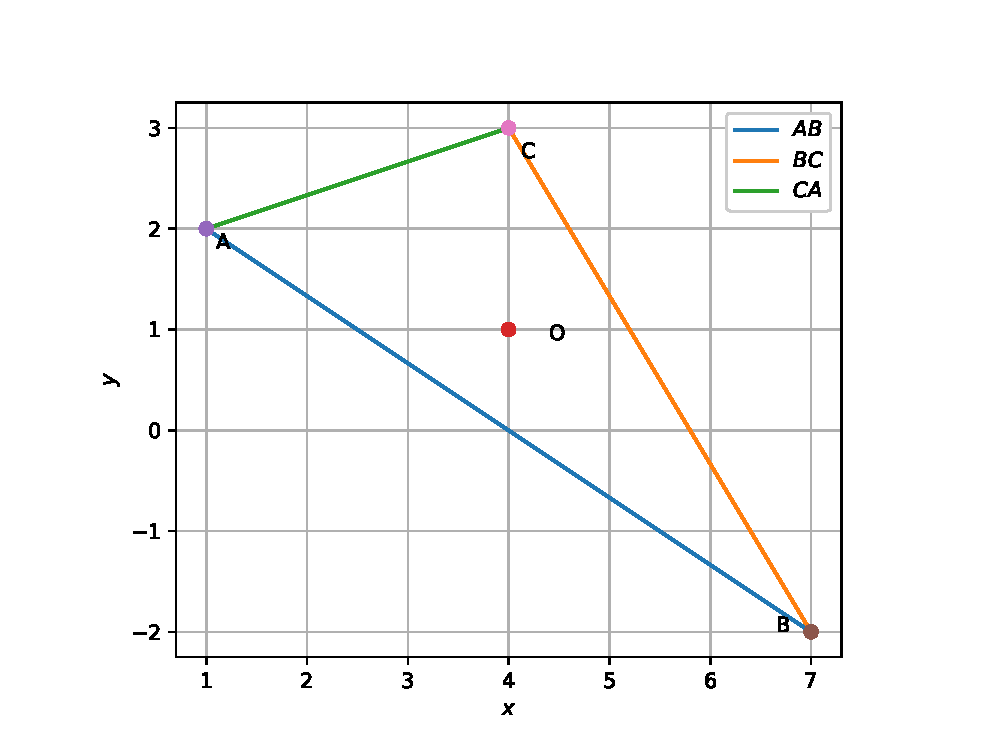
\includegraphics[width=\columnwidth]{./line/figs/triangle.eps}
\caption{}
\label{fig:triangle}
\end{figure}
\end{enumerate}

